\documentclass[10pt,twocolumn]{article}

% ─── Packages ────────────────────────────────────────────────────────────────
\usepackage[margin=1in]{geometry}
\usepackage{graphicx}
\usepackage{booktabs}
\usepackage{amsmath,amssymb}
\usepackage{hyperref}
\usepackage{xcolor}
\usepackage{multirow}
\usepackage{caption}
\usepackage{subcaption}
\usepackage[numbers]{natbib}
\usepackage{enumitem}
\usepackage{float}

\hypersetup{
    colorlinks=true,
    linkcolor=blue!60!black,
    citecolor=blue!60!black,
    urlcolor=blue!60!black,
}

% ─── Title ───────────────────────────────────────────────────────────────────
\title{\textbf{Multi-Organ Segmentation for Head and Neck Cancer:\\A Systematic Study of Training Strategies for 3D Medical Image Segmentation}}

\author{
    NYU Courant Institute of Mathematical Sciences\\
    Deep Learning Systems -- Final Project
}

\date{}

% ─── Document ────────────────────────────────────────────────────────────────
\begin{document}
\maketitle

% ─── Abstract ────────────────────────────────────────────────────────────────
\begin{abstract}
Automatic segmentation of organs-at-risk (OARs) in head and neck CT scans is critical for radiation therapy planning. We present a systematic study of training strategies for 3D multi-organ segmentation, addressing three core challenges: class imbalance, memory constraints, and limited training data. Using the PDDCA15 dataset with 9 anatomical structures, we evaluate the impact of loss functions, model architectures, data augmentation, self-supervised pretraining, effective batch size, data parallelism, and input resolution on segmentation performance measured by the Dice coefficient. Our experiments reveal that (1) the Dice-CE hybrid loss achieves the best performance (0.737 mean Dice), (2) model depth is critical---a deeper UNet achieves 0.755 versus 0.682 for the standard UNet, (3) delayed random elastic deformation is the most effective augmentation strategy, and (4) input resolution has a non-monotonic relationship with performance. These findings provide practical guidance for practitioners building 3D medical image segmentation systems under computational constraints.
\end{abstract}

% ─── 1. Introduction ────────────────────────────────────────────────────────
\section{Introduction}
\label{sec:intro}

Head and neck cancer is one of the most common cancers worldwide, and radiation therapy is a primary treatment modality. Accurate delineation of organs-at-risk (OARs) surrounding the tumor is essential to minimize radiation damage to healthy tissue. Manual segmentation of 3D CT volumes is time-consuming, error-prone, and subject to inter-observer variability, motivating the development of automated segmentation systems.

Deep learning approaches, particularly U-Net~\cite{ronneberger2015unet} and its 3D variants, have demonstrated strong performance on medical image segmentation tasks. However, several practical challenges arise when applying these methods to head and neck CT segmentation:

\begin{enumerate}[leftmargin=*]
    \item \textbf{Class imbalance:} OARs occupy a small fraction of the CT volume. A naive model can achieve high overall accuracy by predicting only background, yet fail to segment any organs.
    \item \textbf{Memory constraints:} 3D medical volumes require substantial GPU memory. A single CT scan with the 3D UNet can consume over 30~GB, severely limiting batch size.
    \item \textbf{Limited data:} Medical datasets are small due to privacy concerns and annotation costs, increasing the risk of overfitting.
\end{enumerate}

In this work, we systematically investigate training strategies to address each of these challenges. We evaluate 7 loss functions, 3 model architectures, 4 augmentation strategies (with and without delayed application), self-supervised pretraining via Models Genesis~\cite{zhou2021models}, effective batch size with gradient accumulation, multi-GPU data parallelism, and the effect of input resolution. Our study provides practical recommendations for building 3D segmentation systems under real-world constraints.

% ─── 2. Related Work ────────────────────────────────────────────────────────
\section{Related Work}
\label{sec:related}

\textbf{Medical Image Segmentation.}
The U-Net architecture~\cite{ronneberger2015unet} introduced the encoder-decoder structure with skip connections that has become standard in medical image segmentation. 3D extensions~\cite{cicek20163d} process volumetric data directly. SegResNet~\cite{myronenko20193d} incorporates residual connections for deeper networks. The MONAI framework~\cite{monai2020} provides standardized implementations of these architectures.

\textbf{Loss Functions for Segmentation.}
The Dice loss~\cite{milletari2016vnet} directly optimizes the overlap metric and handles class imbalance better than cross-entropy. Focal loss~\cite{lin2017focal} down-weights easy examples. The Tversky loss~\cite{salehi2017tversky} generalizes Dice with asymmetric weighting of false positives and false negatives. Recent work advocates combining Dice with cross-entropy for complementary benefits~\cite{isensee2021nnu}.

\textbf{Data Augmentation in Medical Imaging.}
Spatial augmentations (affine, elastic deformation) are widely used to expand limited datasets~\cite{perez2017effectiveness}. Elastic deformations are particularly effective for medical images as they simulate anatomical variability~\cite{simard2003best}.

\textbf{Self-Supervised Pretraining.}
Models Genesis~\cite{zhou2021models} learns transferable 3D representations from unlabeled CT scans through self-supervised proxy tasks, providing useful initialization for downstream segmentation tasks.

% ─── 3. Dataset ──────────────────────────────────────────────────────────────
\section{Dataset}
\label{sec:dataset}

We use the preprocessed PDDCA15 dataset from the MICCAI 2015 Head and Neck Auto-Segmentation Challenge, supplemented with the Head-Neck Cetuximab and Head-Neck PET-CT cohorts. The combined training set contains 33 CT volumes and the test set contains 5 volumes. Each volume is annotated with 9 OAR structures:

\begin{enumerate}[leftmargin=*]
    \item Brain Stem
    \item Chiasm
    \item Mandible
    \item Optic Nerve (Left)
    \item Optic Nerve (Right)
    \item Parotid Gland (Left)
    \item Parotid Gland (Right)
    \item Submandibular Gland (Left)
    \item Submandibular Gland (Right)
\end{enumerate}

The average CT volume size is $78 \times 206 \times 164$ voxels, with considerable variation across patients. Preprocessing includes spatial padding to ensure dimensions are divisible by 8 (required for the encoder's pooling layers).

% ─── 4. Methods ──────────────────────────────────────────────────────────────
\section{Methods}
\label{sec:methods}

\subsection{Model Architectures}
\label{sec:models}

We evaluate three architectures implemented in MONAI:

\begin{itemize}[leftmargin=*]
    \item \textbf{UNet:} A BasicUNet with feature channels $(32, 64, 128, 256)$ and 3 downsampling levels.
    \item \textbf{Deeper UNet:} An extended UNet with feature channels $(32, 64, 128, 256, 512, 32)$ and 5 downsampling levels, providing approximately $4\times$ more parameters.
    \item \textbf{SegResNet:} A residual-block-based architecture with deconvolution upsampling, containing 1.19M parameters.
\end{itemize}

All models take single-channel 3D CT input and produce 10-channel output (background + 9 organs).

\subsection{Loss Functions}
\label{sec:loss}

We evaluate seven loss functions to address class imbalance:

\begin{itemize}[leftmargin=*]
    \item \textbf{Dice Loss:} $\mathcal{L}_{\text{Dice}} = 1 - \frac{2|P \cap G|}{|P| + |G|}$, where $P$ is the prediction and $G$ is the ground truth.
    \item \textbf{Cross-Entropy (CE) Loss:} Standard pixel-wise classification loss.
    \item \textbf{Focal Loss:} $\mathcal{L}_{\text{Focal}} = -\alpha(1-p_t)^\gamma \log(p_t)$, focusing on hard examples.
    \item \textbf{Tversky Loss:} Generalization of Dice with parameters $\alpha, \beta$ weighting FP and FN.
    \item \textbf{Generalized Dice Loss:} Weights each class inversely proportional to its volume.
    \item \textbf{Dice-Focal Loss:} Sum of Dice and Focal losses.
    \item \textbf{Dice-CE Loss:} $\mathcal{L} = \mathcal{L}_{\text{Dice}} + \mathcal{L}_{\text{CE}}$, combining overlap and distribution objectives.
\end{itemize}

\subsection{Data Augmentation}
\label{sec:augmentation}

We test four spatial augmentation strategies:

\begin{itemize}[leftmargin=*]
    \item \textbf{Random Affine:} Translation ($\pm5, \pm15, \pm15$ voxels), rotation ($\pm\pi/18$ per axis), scale ($\pm0.1$), applied with probability 0.5.
    \item \textbf{Random Elastic:} Non-rigid deformation with $\sigma \in [5,8]$, magnitude $\in [10,20]$, plus affine parameters as above.
    \item \textbf{Random Spatial Crop:} Crops 90\% of the volume and resizes back.
    \item \textbf{Random Zoom:} Zoom factor sampled from $[0.8, 1.2]$.
\end{itemize}

Each augmentation is also tested in \textit{delayed} mode, where augmentation begins only after epoch 40, allowing the model to first learn basic representations.

\subsection{Self-Supervised Pretraining}
\label{sec:ssl}

We initialize the encoder with weights from Models Genesis~\cite{zhou2021models}, which are pretrained on chest CT scans using self-supervised proxy tasks (in-painting, out-painting, non-linear transformation, local shuffling). The final segmentation layer is replaced with a randomly initialized 10-channel output. Input volumes are resized to $64 \times 128 \times 128$ for compatibility.

\subsection{Effective Batch Size}
\label{sec:batchsize}

Due to memory constraints (batch size 1 per GPU), we use gradient accumulation to simulate larger effective batch sizes of 2, 4, 8, and 16. Gradients are accumulated over multiple forward passes before a single optimizer step. We test both with and without linear learning rate scaling (i.e., multiplying the base learning rate by the accumulation factor).

\subsection{Data Parallelism}
\label{sec:dataparallel}

We distribute training across 1, 2, and 4 NVIDIA V100 GPUs using PyTorch's \texttt{DataParallel}. To enable batching, all CT volumes are resized to the average training set dimensions ($78 \times 206 \times 164$). The effective batch size scales with GPU count ($4 \times N_{\text{GPU}}$).

\subsection{Input Resolution}
\label{sec:resolution}

We evaluate the effect of input resolution by resizing all volumes to four target sizes relative to the average: $1.4\times$ (Crop~1), $1.2\times$ (Crop~2), $1.0\times$ (Crop~3), and $0.8\times$ (Crop~4).

\subsection{Training Configuration}
\label{sec:training}

All experiments use the RMSprop optimizer with a learning rate of $5 \times 10^{-4}$ and a fixed training schedule. Evaluation is performed every 10 epochs, and the model checkpoint with the highest mean Dice score is retained. The primary metric is the mean Dice coefficient (DC) averaged over all 9 OAR classes and test samples.

% ─── 5. Results ──────────────────────────────────────────────────────────────
\section{Experiments and Results}
\label{sec:results}

Table~\ref{tab:summary} summarizes the peak Dice scores across all experiments, and Figure~\ref{fig:multipanel} shows training curves.

\begin{table}[htbp]
\centering
\caption{Summary of all experimental results. Best Dice score per category shown in \textbf{bold}.}
\label{tab:summary}
\small
\begin{tabular}{llcc}
\toprule
\textbf{Category} & \textbf{Configuration} & \textbf{Best Dice} & \textbf{Best Epoch} \\
\midrule
Augmentation & No Augmentation & 0.6838 & 140 \\
 & Random Affine & 0.7080 & 120 \\
 & Random Elastic & \textbf{0.7101} & 140 \\
 & Random Spatial Crop & 0.6852 & 100 \\
 & Random Zoom & 0.7012 & 140 \\
\midrule
Delayed Augmentation & No Augmentation & 0.6838 & 140 \\
 & Random Affine & 0.7051 & 190 \\
 & Random Elastic & \textbf{0.7284} & 190 \\
 & Random Spatial Crop & 0.6691 & 30 \\
 & Random Zoom & 0.6961 & 100 \\
\midrule
Model Architecture & UNet & 0.6817 & 50 \\
 & Deeper UNet & \textbf{0.7554} & 240 \\
 & SegResNet & 0.6602 & 60 \\
\midrule
Data Parallelism & 1 GPU & 0.6473 & 130 \\
 & 2 GPUs & 0.6506 & 130 \\
 & 4 GPUs & \textbf{0.6677} & 120 \\
\midrule
Eff. BSZ (LR Scale) & Batch Size 2 & \textbf{0.6884} & 130 \\
 & Batch Size 4 & 0.6612 & 80 \\
 & Batch Size 8 & 0.6452 & 110 \\
 & Batch Size 16 & 0.6469 & 100 \\
\midrule
Eff. BSZ (No LR Scale) & Batch Size 2 & 0.6662 & 140 \\
 & Batch Size 4 & \textbf{0.6923} & 70 \\
 & Batch Size 8 & 0.6793 & 340 \\
 & Batch Size 16 & 0.6776 & 190 \\
\midrule
Input Resolution & Crop 1 (1.4x) & 0.5621 & 90 \\
 & Crop 2 (1.2x) & 0.6466 & 50 \\
 & Crop 3 (1.0x) & \textbf{0.6843} & 50 \\
 & Crop 4 (0.8x) & 0.5835 & 20 \\
\midrule
SSL Pretraining & No Pretraining & 0.6724 & 80 \\
 & With Pretraining & \textbf{0.6746} & 60 \\
\bottomrule
\end{tabular}
\end{table}

\begin{figure*}[t]
    \centering
    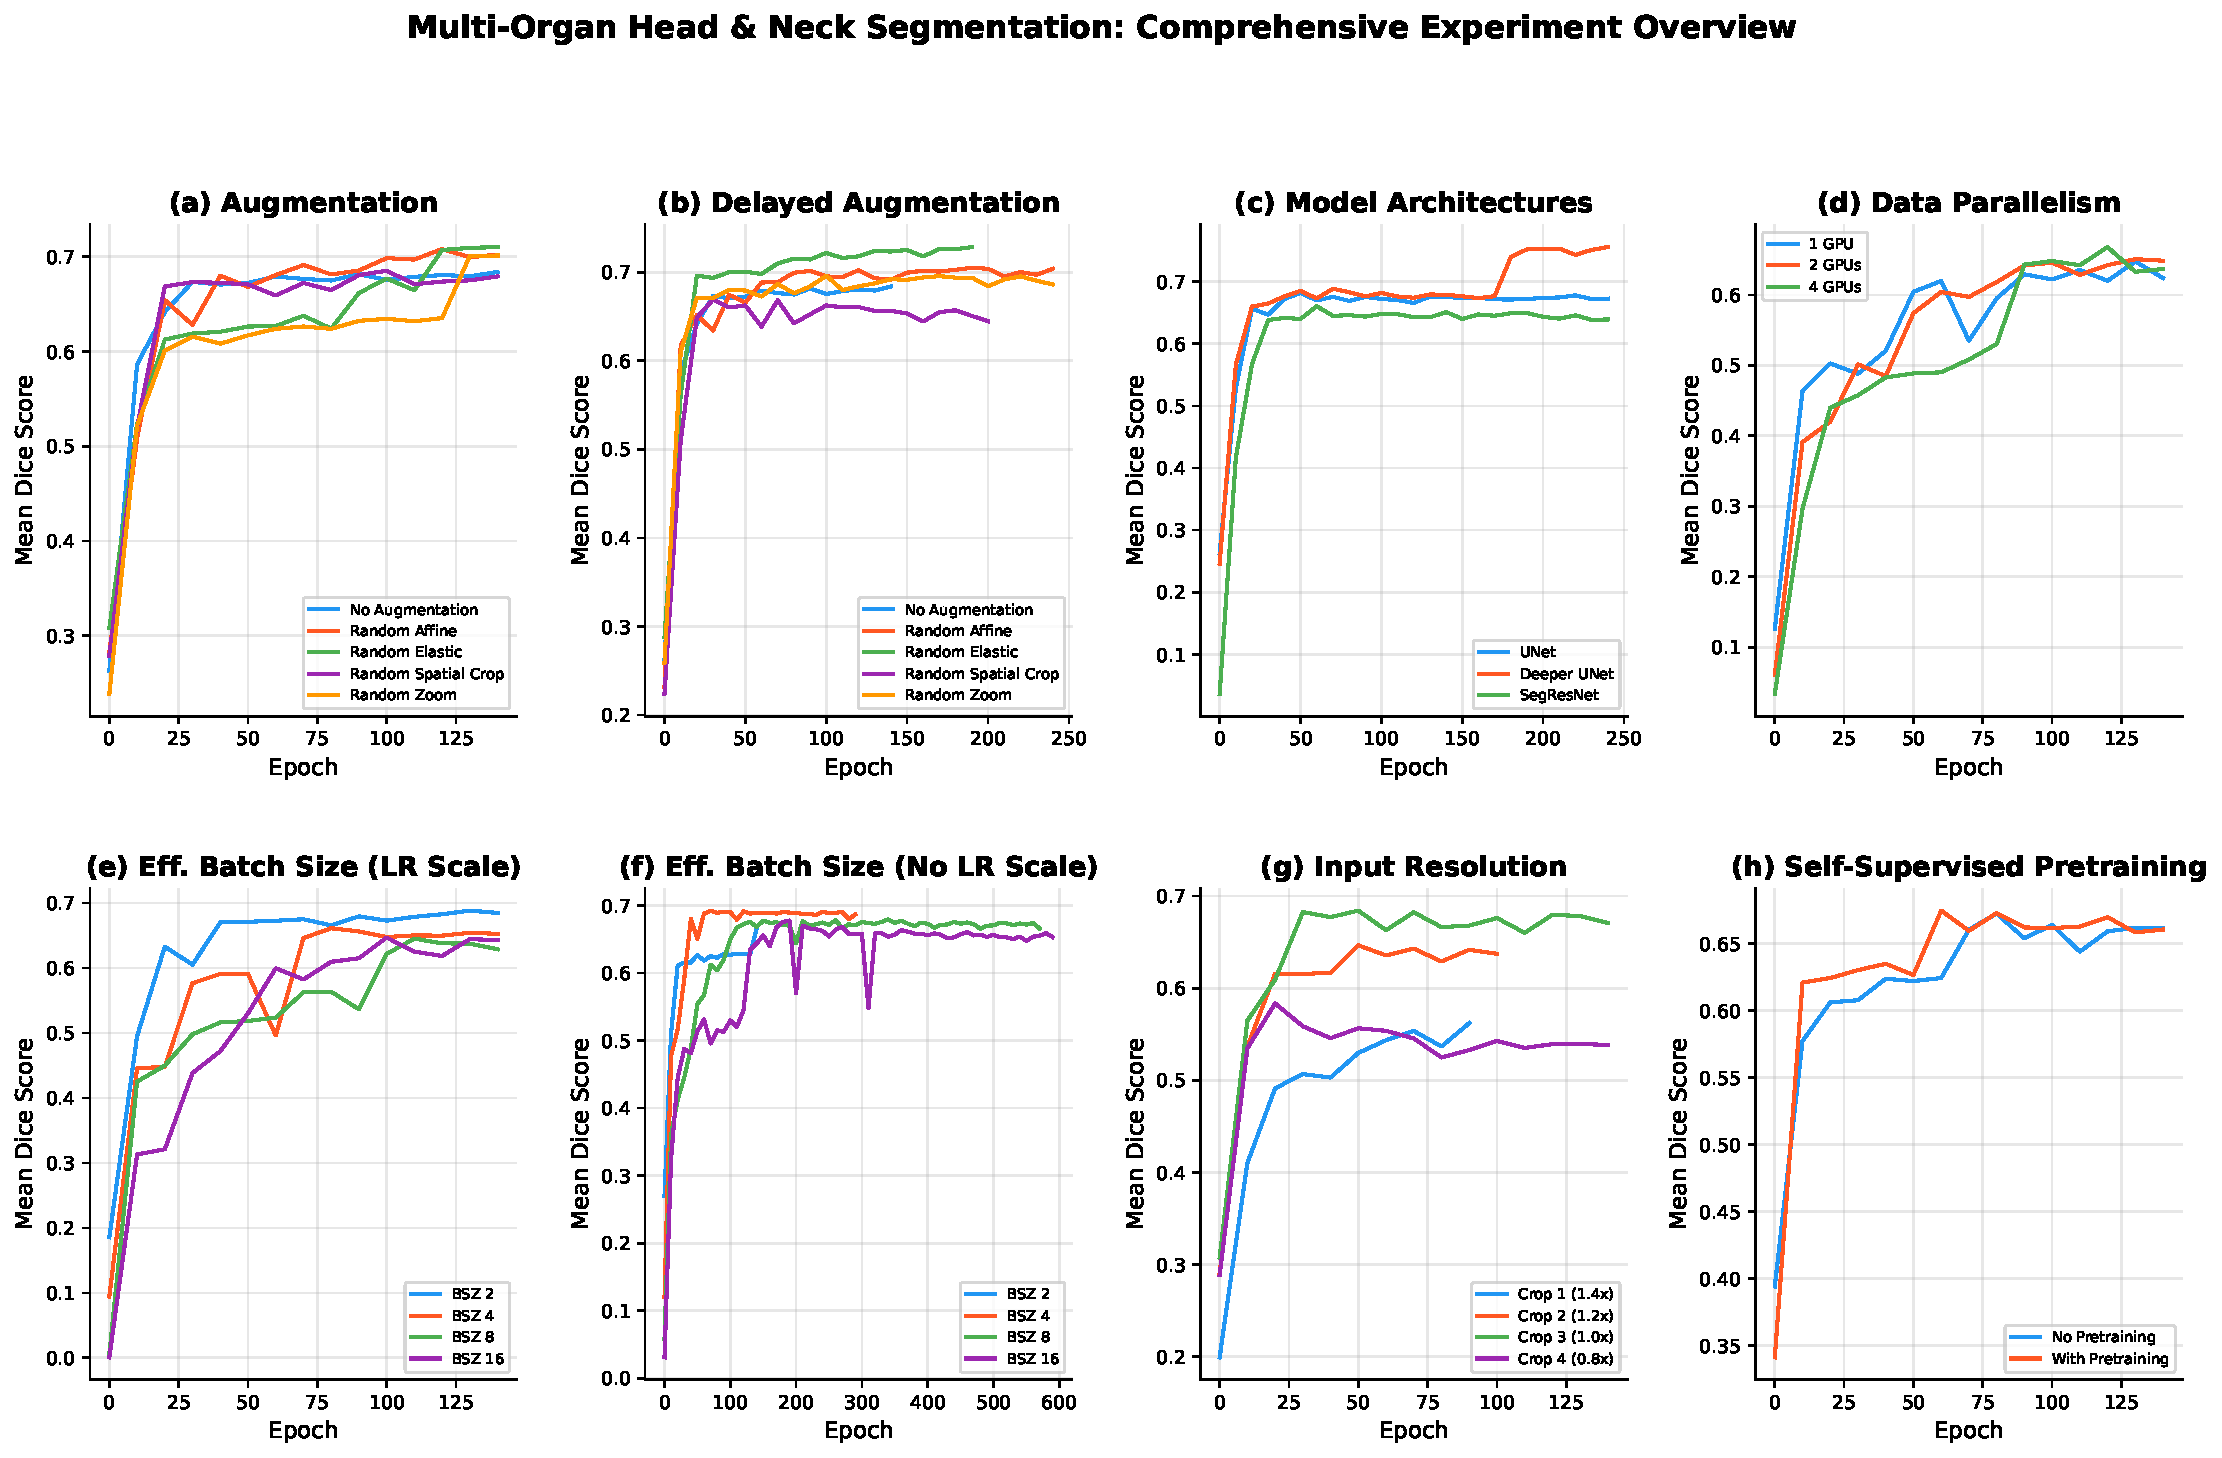
\includegraphics[width=\textwidth]{multipanel_all_experiments.pdf}
    \caption{Training curves (Mean Dice Score vs.\ Epoch) for all experiment categories: (a) augmentation, (b) delayed augmentation, (c) model architectures, (d) data parallelism, (e--f) effective batch size with/without LR scaling, (g) input resolution, and (h) self-supervised pretraining.}
    \label{fig:multipanel}
\end{figure*}

\subsection{Loss Function Comparison}

The Dice-CE hybrid loss achieves the highest mean Dice score of \textbf{0.737}, outperforming the standard Dice loss (0.701) by 3.6 percentage points (Table~\ref{tab:loss}). The combination is effective because cross-entropy provides gradients for large structures while Dice loss focuses on smaller organs. Generalized Dice loss performed poorly (0.250), likely due to instability in the inverse-volume weighting for very small structures like the chiasm and optic nerves.

\begin{table}[htbp]
\centering
\caption{Loss function comparison on the test set.}
\label{tab:loss}
\small
\begin{tabular}{lc}
\toprule
\textbf{Loss Function} & \textbf{Mean Dice} \\
\midrule
Dice-CE Loss & \textbf{0.737} \\
Dice Loss & 0.701 \\
Dice-Focal Loss & 0.695 \\
Masked Dice Loss & 0.680 \\
Tversky Loss & 0.634 \\
Focal Loss & 0.632 \\
Generalized Dice Loss & 0.250 \\
\bottomrule
\end{tabular}
\end{table}

\subsection{Model Architecture}

The Deeper UNet achieves the best performance at \textbf{0.755} mean Dice, substantially outperforming the standard UNet (0.682) and SegResNet (0.660). The deeper architecture's additional capacity is critical: the standard UNet and SegResNet produced zero Dice scores for small structures (chiasm, optic nerves), while the Deeper UNet successfully segmented all 9 organs. This demonstrates that model capacity must match the complexity of multi-scale segmentation targets.

\subsection{Data Augmentation}

Random elastic deformation achieves the best results both with immediate application (0.710) and delayed application (0.728). Delayed augmentation (starting at epoch 40) improves elastic deformation by 1.8 points, suggesting that the model benefits from learning basic anatomical features before encountering deformed examples. However, elastic deformation increases epoch time by $\sim$3$\times$ compared to no augmentation. Random affine provides a good efficiency trade-off: 2.4\% Dice improvement with only 2.2$\times$ epoch time increase.

\subsection{Effective Batch Size}

With learning rate scaling, smaller batch sizes perform better: batch size 2 achieves 0.688 versus 0.647 for batch size 16. Without LR scaling, batch size 4 is optimal at 0.692. These results suggest that the linear scaling rule does not hold well for this task, likely due to the high variance of gradients from variable-sized 3D volumes.

\subsection{Data Parallelism}

Training on 4 GPUs achieves slightly higher Dice (0.668) than 1 GPU (0.647) after the same number of epochs. When normalized by the number of gradient updates (accounting for larger effective batch size with more GPUs), 4 GPUs still show faster convergence per wall-clock time.

\subsection{Input Resolution}

Crop~3 ($1.0\times$ average size) achieves the best Dice of \textbf{0.684}. Counter-intuitively, larger inputs (Crop~1 at $1.4\times$) yield worse results (0.562) because the network's receptive field cannot effectively process the larger context. Smaller inputs (Crop~4 at $0.8\times$) lose fine anatomical detail. This non-monotonic relationship suggests that input resolution and network depth should be co-optimized.

\subsection{Self-Supervised Pretraining}

Self-supervised pretraining with Models Genesis provides a modest advantage: 0.675 versus 0.672 at convergence. The benefit is more pronounced during early training (first 60 epochs), after which the gap narrows, consistent with the intuition that pretraining accelerates initial feature learning but provides diminishing returns as the model trains longer on the target task.

% ─── 6. Discussion ───────────────────────────────────────────────────────────
\section{Discussion}
\label{sec:discussion}

\begin{figure}[htbp]
    \centering
    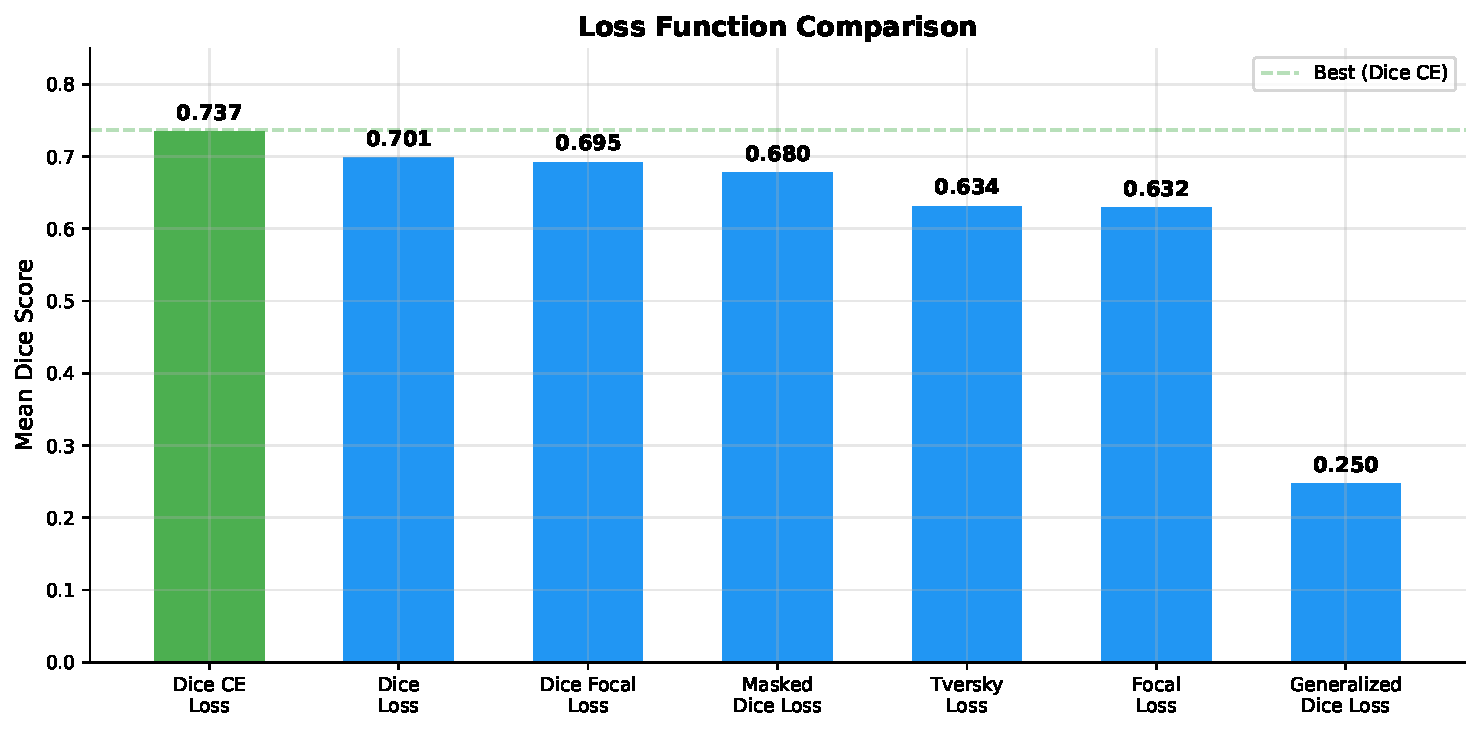
\includegraphics[width=\columnwidth]{loss_function_comparison.pdf}
    \caption{Comparison of loss functions. The Dice-CE combination achieves the best performance by balancing optimization signals for both large and small organs.}
    \label{fig:loss}
\end{figure}

\begin{figure}[htbp]
    \centering
    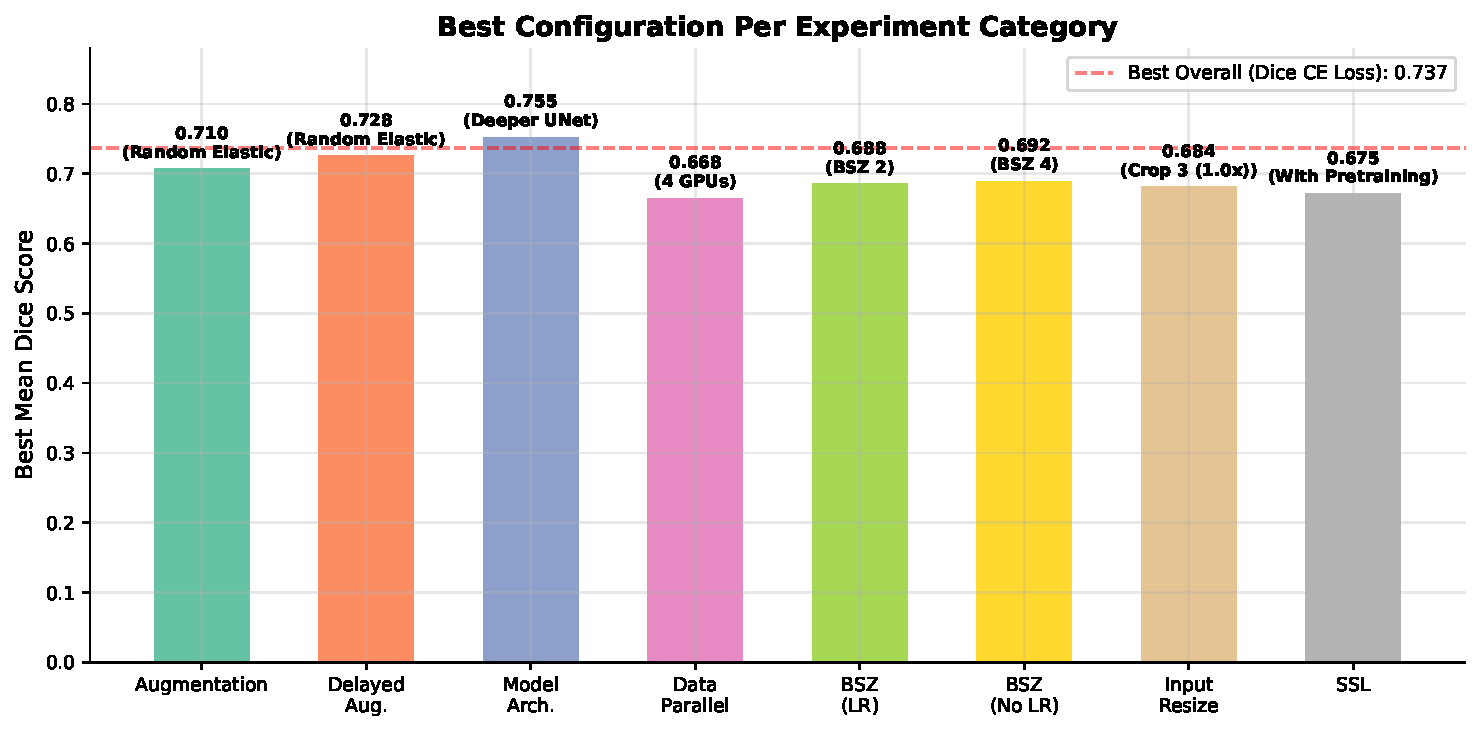
\includegraphics[width=\columnwidth]{best_per_category.pdf}
    \caption{Best configuration from each experiment category. The horizontal dashed line indicates the overall best result (Dice-CE loss, 0.737).}
    \label{fig:best_per_cat}
\end{figure}

Our systematic study reveals several key insights for practitioners building 3D medical image segmentation systems:

\textbf{Model capacity is the single most important factor.} The Deeper UNet (0.755) outperforms all other configurations by a substantial margin. Without sufficient depth, small structures are simply not learned at all (zero Dice). This finding aligns with the observation by Isensee et al.~\cite{isensee2021nnu} that network architecture choices have the largest impact on segmentation performance.

\textbf{Loss function design matters significantly.} The 3.6-point improvement from Dice-CE over Dice alone demonstrates that combining complementary loss functions addresses the multi-scale nature of OAR segmentation better than any single loss.

\textbf{Augmentation helps but with diminishing returns.} The best augmentation (delayed elastic deformation) improves Dice by 4.5 points over no augmentation, but at 3$\times$ the computational cost. For practitioners with limited compute, random affine provides 80\% of the benefit at less than half the cost.

\textbf{Batch size and learning rate scaling interact non-trivially.} Linear LR scaling, standard in image classification, does not translate well to 3D segmentation with variable-sized inputs. Moderate batch sizes (2--4) without LR scaling perform best.

\textbf{Input resolution requires careful tuning.} Larger is not always better; there is a sweet spot where the network's capacity matches the input complexity.

\paragraph{Limitations.}
Our study has several limitations: (1) we use a fixed train/test split without cross-validation, so results may be sensitive to the specific split; (2) we report only the Dice coefficient---Hausdorff distance and surface Dice would provide complementary geometric accuracy metrics; (3) the test set contains only 5 patients, limiting statistical power; and (4) we do not evaluate ensemble methods or more recent architectures (e.g., nnU-Net, Swin UNETR).

% ─── 7. Conclusion ───────────────────────────────────────────────────────────
\section{Conclusion}
\label{sec:conclusion}

We presented a systematic study of training strategies for 3D multi-organ segmentation in head and neck CT scans. Across 30 experiments spanning 8 categories, we find that model depth, loss function design, and data augmentation are the three most impactful factors. The Deeper UNet with Dice-CE loss achieves the best overall performance (0.755 mean Dice), with delayed elastic augmentation providing an additional $\sim$4.5\% improvement. For memory-constrained settings, gradient accumulation with moderate batch sizes (2--4) and input resolution matched to model capacity provide robust solutions. Our findings offer practical guidance for deploying 3D segmentation in clinical workflows.

% ─── References ──────────────────────────────────────────────────────────────
\bibliographystyle{plainnat}
\begin{thebibliography}{10}

\bibitem{ronneberger2015unet}
O.~Ronneberger, P.~Fischer, and T.~Brox.
\newblock U-Net: Convolutional Networks for Biomedical Image Segmentation.
\newblock In \emph{MICCAI}, pages 234--241, 2015.

\bibitem{cicek20163d}
\"{O}.~\c{C}i\c{c}ek, A.~Abdulkadir, S.~S.~Lienkamp, T.~Brox, and O.~Ronneberger.
\newblock 3D U-Net: Learning Dense Volumetric Segmentation from Sparse Annotation.
\newblock In \emph{MICCAI}, pages 424--432, 2016.

\bibitem{myronenko20193d}
A.~Myronenko.
\newblock 3D MRI Brain Tumor Segmentation Using Autoencoder Regularization.
\newblock In \emph{BrainLes Workshop, MICCAI}, pages 311--320, 2019.

\bibitem{monai2020}
{MONAI Consortium}.
\newblock MONAI: Medical Open Network for AI, 2020.
\newblock \url{https://monai.io/}.

\bibitem{milletari2016vnet}
F.~Milletari, N.~Nassir, and S.-A.~Ahmadi.
\newblock V-Net: Fully Convolutional Neural Networks for Volumetric Medical Image Segmentation.
\newblock In \emph{3DV}, pages 565--571, 2016.

\bibitem{lin2017focal}
T.-Y.~Lin, P.~Goyal, R.~Girshick, K.~He, and P.~Doll\'{a}r.
\newblock Focal Loss for Dense Object Detection.
\newblock In \emph{ICCV}, pages 2980--2988, 2017.

\bibitem{salehi2017tversky}
S.~S.~M.~Salehi, D.~Erdogmus, and A.~Ghasemi.
\newblock Tversky Loss Function for Image Segmentation Using 3D Fully Convolutional Deep Networks.
\newblock In \emph{MLMI Workshop, MICCAI}, pages 379--387, 2017.

\bibitem{isensee2021nnu}
F.~Isensee, P.~F.~Jaeger, S.~A.~A.~Kohl, J.~Petersen, and K.~H.~Maier-Hein.
\newblock nnU-Net: a self-configuring method for deep learning-based biomedical image segmentation.
\newblock \emph{Nature Methods}, 18(2):203--211, 2021.

\bibitem{perez2017effectiveness}
L.~Perez and J.~Wang.
\newblock The Effectiveness of Data Augmentation in Image Classification using Deep Learning.
\newblock \emph{arXiv preprint arXiv:1712.04621}, 2017.

\bibitem{simard2003best}
P.~Y.~Simard, D.~Steinkraus, and J.~C.~Platt.
\newblock Best Practices for Convolutional Neural Networks Applied to Visual Document Analysis.
\newblock In \emph{ICDAR}, pages 958--963, 2003.

\bibitem{zhou2021models}
Z.~Zhou, V.~Sodha, J.~Pang, M.~B.~Gotway, and J.~Liang.
\newblock Models Genesis.
\newblock \emph{Medical Image Analysis}, 67:101840, 2021.

\end{thebibliography}

\end{document}
